\subsection{Teil 2 - Informationsextraktion}
\label{chap:ie}

% https://www.diva-portal.org/smash/get/diva2:934351/FULLTEXT01.pdf
% -> Referenziert System von Hamza et al.
% -> OCR Error Correction approach von Sorio et al.


Um eine Rechnung verarbeiten zu können, müssen Informationen, wie beispielsweise der Totalbetrag oder der Leistungsbezüger, aus dieser extrahiert werden. Eine Lösung zu dieser Problematik der Informationsextraktion wird bereits von vielen existieren Softwarelösungen zur automatisierten Verarbeitung von Rechnungen angeboten. Solche Systeme extrahieren zwei verschiedene Typen von Informationen: Informationen mit Schlüsselwörter und Informationen aus Tabellen~\autocite{Hamza}.

Zur Extraktion von Informationen aus Tabellen sind viele Ansätze in der Literatur zu finden. Ein einfacher Ansatz von \textcite{Mandal} erreicht bereits eine Trefferquote von 97.21\%~(\cite{Mandal} in \cite{Hamza}).

\textcite{Hamza} stellen eine Lösung zur Informationsextraktion aus Rechnungen vor, welche mit Hilfe von Case Based Reasoning\footnote{Unter Case Based Reasoning, kurz CBR, werden Ansätze verstanden, bei welchen Entscheidungen aufgrund vergangener Erfahrungen getroffen werden. Die Theorie des Case Based Reasoning sieht das Treffen von Entscheidungen aufgrund von Analogien als zentralen Aspekt der menschlichen Intelligenz und versucht diesen in die künstliche Intelligenz einzubringen~\autocite{CBR}.}, eine Trefferquote von 76-85\% erreicht. Knapp die Hälfte der Fehler wird dabei durch OCR Fehler verursacht.

Im Gegensatz zu den diskutierten Lösungen ist in diesem Experiment die Extraktion von Informationen aus Tabellen nicht relevant. Für die Verarbeitung der Rechnungen im vorliegenden Fallbeispiel ist die Extraktion einzelner Rechnungspositionen ebenfalls nicht relevant.

In den folgenden Kapiteln werden zwei Lösungsvorschläge zur Extraktion von Informationen aus Rechnungen diskutiert. Die gewählten Ansätze sind, verglichen zu den oben erwähnten Ansätzen von \textcite{Mandal} und \textcite{Hamza}, einfach gehalten. 

Der erste Ansatz stammt aus einem Joint Venture zwischen der AXA, der 3AP AG und der Fachhochschule Nordwestschweiz. Der zweite Ansatz wurde im Rahmen dieser Arbeit erarbeitet.

\subsubsection{Bild-basierte Informationsextraktion}

In diesem Kapitel wird ein bild-basierter Ansatz zur Informationsextraktion aus Rechnungen vorgestellt. Der Ansatz stammt aus einem Joint Ventrue zwischen der AXA, der 3AP AG und der Fachhochschule Nordwestschweiz. 

Auch dieser bild-basierte Ansatz basiert, analog dem bild-basierten Ansatz zur Klassifizierung, auf Algorithmen und Modellen aus dem Bereich der Computer-Vision.

Der präsentierte Ansatz basiert auf der Idee, Modelle, welche ursprünglich zur Objekterkennung in Bildern entwickelt wurden, zur Erkennung von Regionen mit relevanten Informationen (Region of Interest) zu verwenden. Konkret bedeutet dies, dass mit einem Modell zur Objekterkennung die Positionen der Adresse des Patienten, des Namens des Leistungserbringers, der Rechnungspositionen sowie des Totalbetrages auf den Rechnungen identifiziert werden sollen. Die Abbildung \ref{fig:roi-example} zeigt zwei Rechnungen, welche manuell mit den erwarteten Regions of Interest annotiert wurden. Dabei wurden persönliche Daten aus Datenschutzgründen unkenntlich gemacht.

\begin{figure}[H]
  \captionsetup{width=.9\linewidth}
  \caption{Zwei Beispiele von Rechnungen mit annotierten Regions of Interest}
  \label{fig:roi-example}
  \centering
  \begin{subfigure}[t]{0.5\linewidth}
    \captionsetup{width=.9\linewidth}
    \centering
    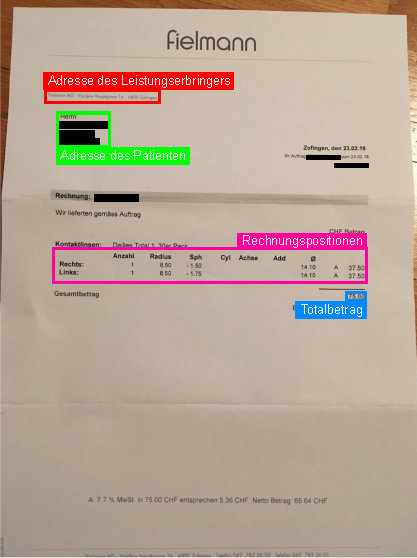
\includegraphics[scale=1]{graphics/roi-example-cp.pdf}
    \vspace{6pt}
    \subcaption{Eine über das Kundenportal eingereichte Rechnung} 
    \vspace{2ex}
  \end{subfigure}%% 
  \begin{subfigure}[t]{0.5\linewidth}
    \captionsetup{width=.9\linewidth}
    \centering
    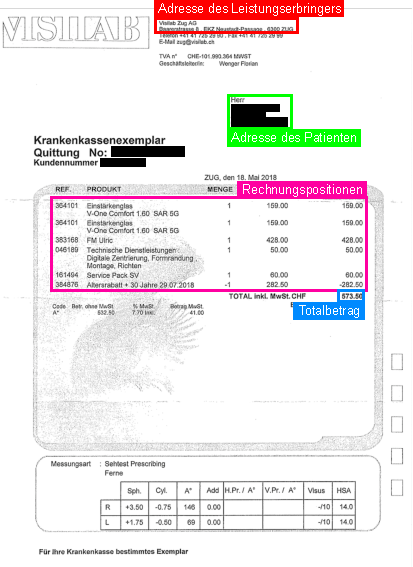
\includegraphics[scale=1]{graphics/roi-example-scan.pdf}
    \subcaption{Eine via Post eingereichte Rechnung} 
    \vspace{2ex}
  \end{subfigure}
\end{figure}

Dieser Ansatz wurde mit dem Framework luminoth umgesetzt. Dabei steht das Single-Shot Multibox Detector (SSD) sowie das Faster-RCNN Modell zur Verfügung. Das SSD Modell ist eines der performantesten Modelle zur Objekterkennung. Das Faster-RCNN Modell ist aktuell eines der präzisesten, aber dafür rechenintensivsten, Modelle~\autocite{SSDFRCNN}.

Die beiden Modelle werden auf einem Datensatz von knapp 900 Rechnungen von Optikern trainiert. Diese Rechnungen wurden manuell mit den Regions of Interest annotiert.

Die Abbildungen \ref{fig:3ap-map:map_train} und \ref{fig:3ap-map:map_val} zeigen drei verschiedene Mean Average Precision Metriken der beiden Modelle auf den Trainings- respektive Testsdaten. In Abbildung \ref{fig:3ap-map:map_val} ist zu sehen, dass das Faster-RCNN Modell nach knapp 1'500 Trainingsschritten präziser ist als das SSD Modell. Die Mean Average Precision des Faster-RCNN Modell steigt bei einem IoU Schwellenwert von 0.5 bis auf 0.82. Bei einem IoU Schwellwert von 0.75 beziehungsweise $[0.5:0.95]$ steigt die Mean Average Precision nur knapp über respektive bis knapp unter 0.5. Dies bedeutet, dass die Modelle ungefähr erkennen, wo die relevanten Informationen sind, diese aber nicht genau umrahmen können.

Beim Vergleich der Mean Average Precisions auf den Trainings- und Testdaten ist zu erkennen, dass die Modelle ein hohes Bias aufweisen. Es ist bereits während dem Training eine starke Abweichung von der optimalen Mean Average Precision von 1 zu erkennen. Gegenüber dem Trainingsdatensatz ist die Mean Average Precision auf dem Testdatensatz nur gering kleiner, die Modelle besitzen also eine kleine Varianz. Dies bedeutet, dass die Herkunft der Fehler beim Design der Modelle liegen dürfte und mit mehr Trainingsdaten nicht behoben werden kann. 

\begin{figure}[H]
  \captionsetup{width=.9\linewidth}
  \caption{Average Precision auf den Trainings- und Testdaten des Faster-RCNN und SSD Modells}
  \label{fig:3ap-map}
  \centering
  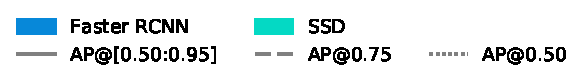
\includegraphics[scale=1]{graphics/matplot/img-detection__legend_3.pdf}
  \begin{subfigure}[t]{0.5\linewidth}
    \centering
    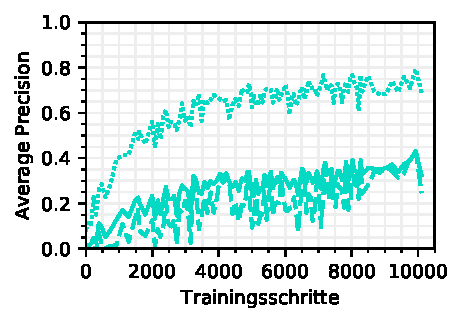
\includegraphics[scale=1]{graphics/matplot/img-detection__all__ap__train.pdf}
    \subcaption{Average Precision auf den Trainingsdaten} 
    \label{fig:3ap-map:map_train}
    \vspace{2ex}
  \end{subfigure}%% 
  \begin{subfigure}[t]{0.5\linewidth}
    \centering
    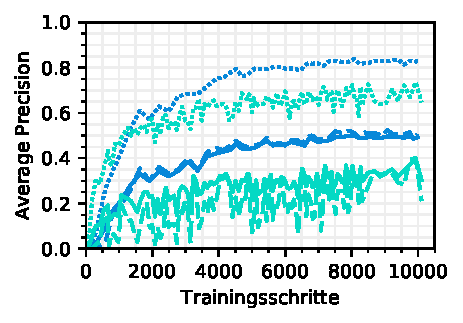
\includegraphics[scale=1]{graphics/matplot/img-detection__all__ap.pdf}
    \subcaption{Average Precision auf den Testdaten} 
    \label{fig:3ap-map:map_val}
    \vspace{2ex}
  \end{subfigure}
\end{figure}

Abbildung \ref{fig:3ap-map:loss} zeigt das Loss der beiden Modelle auf den Testdaten über den Trainingsverlauf hinweg. Es ist zu erkennen, dass das Loss nach 4'000 Trainingsschritten schon sehr flach wird. Die Modelle lernen zu diesem Zeitpunkt also nur noch sehr wenig. Die Modelle noch weiter zu trainieren, würde keine Verbesserung der Mean Average Precision zur Folge haben.

\begin{figure}[h!] 
%\begin{wrapfigure}{r}{0.5\textwidth} 
    \captionsetup{width=.9\linewidth}
    \caption{Totales Loss auf den Testdaten}
    \label{fig:3ap-map:loss}
    \centering
    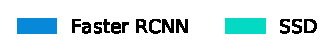
\includegraphics[scale=1]{graphics/matplot/img-detection__legend_1.pdf}
    
    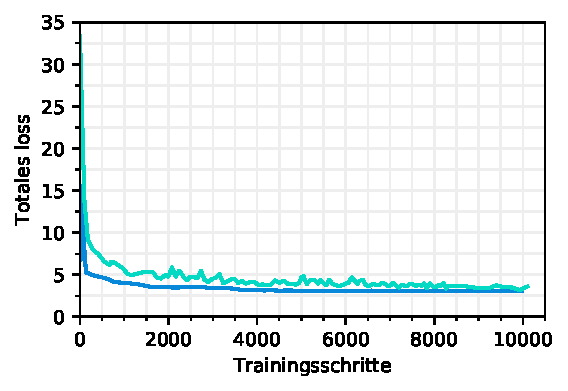
\includegraphics[scale=1]{graphics/matplot/img-detection__all__loss.pdf}
%\end{wrapfigure}
\end{figure}

Einen detaillierteren Einblick in die Qualität der Modelle gibt die Tabelle \ref{tab:3ap-iou}. Die Tabelle zeigt die durchschnittliche Intersection over Union der beiden Modelle für die einzelnen zu erkennenden Klassen. Dabei ist festzustellen, dass die beiden Modelle die Adresse des Patienten sowie die Rechnungspositionen relativ gut erkennen können. Bei den anderen beiden Klassen sind die Resultate dagegen ernüchternd.

Auffällig bei der Gegenüberstellung der Mean IoU Werte ist die Klasse Totalbetrag. Dabei schneidet das SSD Modell extrem schlecht ab. Das SSD Modell scheint mit diesen kleinen Regions of Interest besonders Probleme zu haben.

\begin{table}[h!]
    \centering
    \captionsetup{width=.9\linewidth}
    \caption{Durchschnittliche Intersection over Union der einzelnen Klassen}
    \label{tab:3ap-iou}
    \begin{tabular}{|l|l|l|}
    \hhline{~|--|}    
    \multicolumn{1}{c|}{}
                                    & \multicolumn{2}{c|}{\cellcolor[HTML]{C0E5FD}\textbf{Modell}}  \\
    \hline
    \rowcolor[HTML]{C0E5FD}
    \textbf{Klasse}                 & \textbf{Faster-RCNN} & \textbf{SSD}           \\
    \hline
    Adresse des Patienten           & 0.850       & 0.731         \\
    \hline
    Adresse des Leistungserbringers & 0.625       & 0.623         \\
    \hline
    Rechnungspositionen             & 0.835       & 0.728         \\
    \hline
    Totalbetrag                     & 0.629       & 0.258         \\  
    \hline
    \end{tabular}
\end{table}

Subsummierend kann festgehalten werden, dass das Faster-RCNN Modell erwartungsgemäss präzisere Vorhersagen macht. 

In Bezug auf die Automatisierung der Rechnungseinreichung sind die Adresse des Patienten sowie das Total der Rechnung relevant. Das präsentierte Modell kann aber nur eine der beiden Informationen mit hoher Genauigkeit erkennen. Weiter fehlen andere relevante Informationen wie das Datum des Bezuges der Leistung sowie die Aussage, ob eine ärztliche Verordnung vorliegt oder nicht. 

Im folgenden Kapitel wird versucht diesen Ansatz um die fehlenden Informationen zu ergänzen sowie die Qualität der Ergebnisse zu steigern, indem das Modell auf Rechnungen bestimmter Leistungserbringer spezialisiert wird.

\subsubsection{Bild-basierte Informationsextraktion pro Rechnungstyp}
\label{chap:lerb-specific-ie}

In diesem Kapitel wird der bild-basierte Ansatz zur Informationsextraktion, welcher im vorherigen Kapitel beschrieben wurde, auf Rechnungen eines einzelnen Leistungserbringers (beispielsweise Fielmann) angewendet. Dadurch soll ein besseres Resultat erzielt werden. Des Weiteren werden die zu erkennenden Regions of Interest so angepasst, dass sich diese mit den Anforderungen aus dem Kapitel \ref{chap:requirements} decken. Das bedeutet, dass neu die Positionen der Klassen Adresse des Patienten, Adresse des Leistungserbringers, Datum des Leistungsbezuges, Totalbetrag und Begründung des Leistungsbezuges (mögliche ärztliche Verschreibung) erkannt werden sollen.

Damit in der Praxis spezifische Modelle zur Informationsextraktion auf die Rechnungen der einzelnen Leistungserbringer angewendet werden können, muss das Modell zur Klassifizierung der Rechnung um die Klassen dieser Leistungserbringer erweitert werden. Nachfolgend wird diese Erweiterung des Modells zur Klassifizierung sowie die Erstellung des Leistungserbringer-spezifischen bild-basierten Modell zur Informationsextraktion beschrieben und die Resultate daraus diskutiert.

Das im Kapitel \ref{chap:text-based-classification} beschriebene, text-basierte Modell zur Klassifizierung der Rechnungen wurde um die Klassen Fielmann und Visilab erweitert. Diese Klassen wurden gewählt, da sie innerhalb der aktuell grössten Klasse von Rechnungen, der Klasse Optiker, einen grossen Anteil haben. Es stehen 578 Rechnungen von Fielmann sowie 195 Rechnungen von Visilab zur Verfügung.

Die Abbildung \ref{fielmann-cm} zeigt die Confusion Matrix des angepassten Modells auf den Testdaten. Darauf ist zu erkennen, dass die Einteilung in die beiden neuen Klassen sehr gut funktioniert. Nach 45 Epochen Training werden innerhalb des Testdatensatzes lediglich 2 Rechnungen fälschlicherweise als Rechnungen von Visilab klassifiziert. Diese Klassifizierung ist nicht ganz falsch, denn es handelt sich tatsächlich um Rechnungen von Visilab, aber in einem anderen Format. Es handlet sich um ein Kassenbeleg sowie eine Monatsrechnung. Diese Unterschiede im Format würden nicht in das erwartete Muster des im zweiten Schritt folgenden Modell zur Informationsextraktion passen und werden deshalb als falsch angesehen.

\begin{figure}[h!] 
%\begin{wrapfigure}{r}{0.5\textwidth} 
    \captionsetup{width=.9\linewidth}
    \caption{Confusion Matrix nach 45 Trainingsepochen des erweiterten Text-basierten Modells zur Klassifizierung von Rechnungen}
    \label{fielmann-cm}
    \centering
    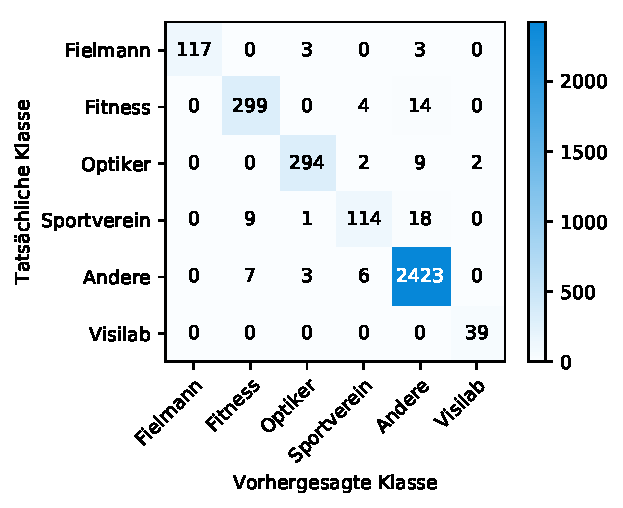
\includegraphics[scale=1]{graphics/matplot/class__fielmann__cm_44.pdf}
%\end{wrapfigure}
\end{figure}

Die Klassifizierung der Rechnungen nach einzelnen Leistungserbringer scheint für das Modell kein Problem darzustellen. Im Folgenden wird nun die Erkennung der Regions of Interest mit dem bild-basierten Ansatz evaluiert.

Das Faster-RCNN und SSD Modell wurden auf den Rechnungen der Klassen Fielmann und Visilab trainiert. Die Abbildung \ref{fig:specific-ie} zeigt die Mean Average Precisions der beiden Modelle für verschiedene IoU Schwellenwerte für die beiden Klassen.

\begin{figure}[h!] 
  \captionsetup{width=.9\linewidth}
  \caption{Average Precision auf den Trainings- und Testdaten der Leistungserbringer spezifischen Modelle}
  \label{fig:specific-ie}
  \centering
  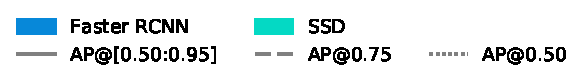
\includegraphics[scale=1]{graphics/matplot/img-detection__legend_3.pdf}
  \begin{subfigure}[b]{0.5\linewidth}
    \captionsetup{width=.9\linewidth}
    \centering
    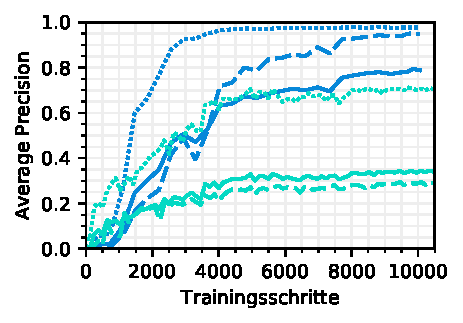
\includegraphics[scale=1]{graphics/matplot/img-detection__fielmann__ap__train.pdf}
    \caption{Average Precision auf den Trainingsdaten der Klasse Fielmann} 
    \label{fig:specific-ie:fielmann:ap_train}
    \vspace{2ex}
  \end{subfigure}%% 
  \begin{subfigure}[b]{0.5\linewidth}
    \captionsetup{width=.9\linewidth}
    \centering
    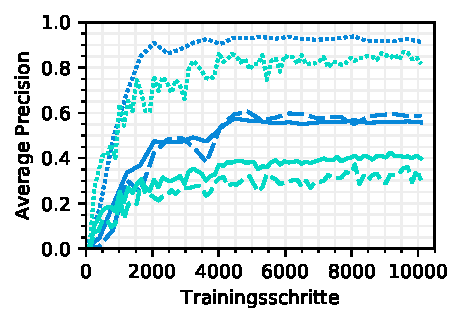
\includegraphics[scale=1]{graphics/matplot/img-detection__visilab__ap.pdf}
    \caption{Average Precision auf den Trainingsdaten der Klasse Visilab} 
    \label{fig:specific-ie:visilab:ap_train}
    \vspace{2ex}
  \end{subfigure}
  \begin{subfigure}[b]{0.5\linewidth}
    \captionsetup{width=.9\linewidth}
    \centering
    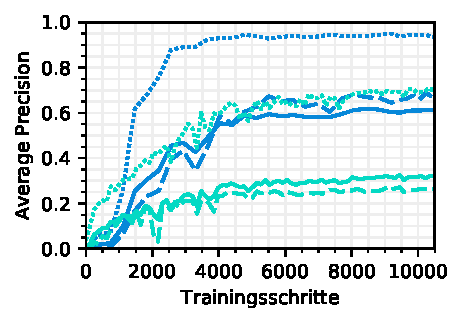
\includegraphics[scale=1]{graphics/matplot/img-detection__fielmann__ap.pdf}
    \caption{Average Precision auf den Testdaten der Klasse Fielmann} 
    \label{fig:specific-ie:fielmann:ap_val}
    \vspace{2ex}
  \end{subfigure}%%
  \begin{subfigure}[b]{0.5\linewidth}
    \captionsetup{width=.9\linewidth}
    \centering
    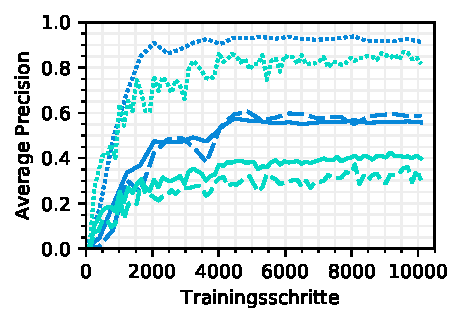
\includegraphics[scale=1]{graphics/matplot/img-detection__visilab__ap.pdf}
    \caption{Average Precision auf den Testdaten der Klasse Visilab} 
    \label{fig:specific-ie:visilab:ap_val}
    \vspace{2ex}
  \end{subfigure}
\end{figure}

Die Abbildung \ref{fig:specific-ie} zeigt, dass bei den Leistungserbringer spezifischen Modellen der Unterschied in den Mean Average Precisions zwischen dem SSD und Faster-RCNN noch stärker ausfallen (vgl. Abbildung \ref{fig:3ap-map}).

Die Abbildungen \ref{fig:specific-ie:fielmann:ap_train} und \ref{fig:specific-ie:fielmann:ap_val} zeigen die Mean Average Precision des Modells zur Informationsextraktion aus Rechnungen von Fielmann. Das Modell erreicht während dem Training und dem Testen eine beachtliche Mean Average Precision von 98\% respektive 94\% bei einem IoU Schwellwert von 0.5. Das Modell erkennt also für sehr viele Rechnungen, wo sich die Regions of Interest befinden. Die mAP@[0.50:0.95] von 80\% während dem Training zeigt, dass das Modell die Regions relativ genau lokalisiert. Auf dem Testdatensatz liegt die mAP@[0.5:0.95] dagegen bei nur knapp 60\%. Das Modell weist somit bei der mAP@0.5 und mAP@[0.5:0.95] eine Varianz von 4\% respektive 20\% auf. Aus dieser teilweise grossen Varianz ist zu schliessen, dass das Modell mehr Trainingsdaten bedarf, welche jedoch zum aktuellen Zeitpunkt nicht zur Verfügung stehen.

Der Bedarf an mehr Trainingsdaten zeigt, dass ein solcher Ansatz nicht für alle Leistungserbringer realistisch ist. Für viele Leistungserbringer stehen weniger Trainingsdaten zur Verfügung. Diese Problematik manifestiert sich auch bei der Erkennung der Regions of Interest für Rechnungen von Visilab. Mit 195 Rechnungen stehen hier nur rund ein Drittel so viele Rechnungen wie von Fielmann zur Verfügung. Wie in den Abbildungen \ref{fig:specific-ie:visilab:ap_train} und \ref{fig:specific-ie:visilab:ap_val} zu sehen ist, liegt die Varianz der \textit{mAP@[0.5:0.95]} des Faster-RCNN Modells für Rechnungen von Visilab bei knapp 40\%. Dies ist ein klarer Indikator dafür, dass zu wenige Trainingsdaten zur Verfügung stehen.

Die Abbildungen \ref{fig:specific-ie:fielmann:loss} und \ref{fig:specific-ie:visilab:loss} zeigen das Loss der beiden Modelle auf den Testdaten für beide Klassen. Es ist zu erkennen, dass die Modelle auf den Leistungserbringer spezifischen Rechnungen nach ungefähr 4'000 Trainingsschritten nicht mehr lernen. Die Modelle auf den vorliegenden Trainingsdaten weiter zu trainieren, dürfte auch hier keine Erhöhung der Mean Average Precisions mehr zur Folge haben.

\begin{figure}[h!] 
  \captionsetup{width=.9\linewidth}
  \label{fig:specific-ie:loss}
  \caption{Totales Loss auf den Testdaten der Leistungserbringer spezifischen Modelle}
  \centering
  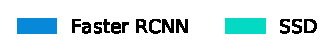
\includegraphics[scale=1]{graphics/matplot/img-detection__legend_1.pdf}
  \begin{subfigure}[b]{0.5\linewidth}
    \captionsetup{width=.9\linewidth}
    \centering
    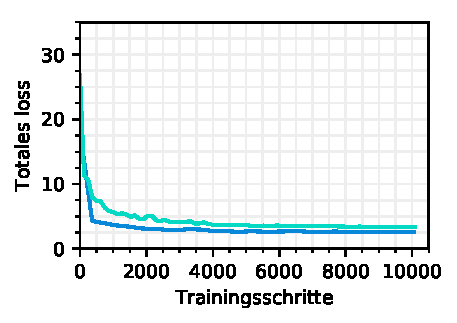
\includegraphics[scale=1]{graphics/matplot/img-detection__fielmann__loss.pdf}
    \caption{Totales Loss auf den Testdaten der Klasse Fielmann} 
    \label{fig:specific-ie:fielmann:loss}
    \vspace{2ex}
  \end{subfigure}%% 
  \begin{subfigure}[b]{0.5\linewidth}
    \captionsetup{width=.9\linewidth}
    \centering
    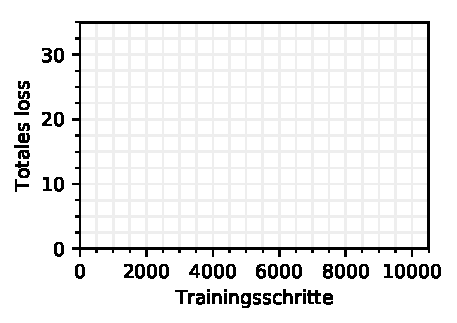
\includegraphics[scale=1]{graphics/matplot/img-detection__visilab__loss.pdf}
    \caption{Totales Loss auf den Testdaten der Klasse Visilab} 
    \label{fig:specific-ie:visilab:loss}
    \vspace{2ex}
  \end{subfigure} 
\end{figure}

Die Tabelle \ref{tab:specific-ie-iou} zeigt die durchschnittliche Intersection over Union für die einzelnen Klassen. Es ist zu erkennen, dass das Faster-RCNN Modell deutlich bessere Resultate liefert als das SSD Modell. Erwähnenswert ist, dass das SSD Modell für die Klasse Behandlungsdatum der Rechnungen von Fielmann überhaupt keine und für den Totalbetrag der Visilab Klasse nur sehr schlechte Regions of Interest vorhersagt. Bei diesen beiden Fällen handelt es sich um kleine Regions mit anderen Regions in unmittelbarer Nähe.

Die Klasse Begründung des Leistungsbezugs ist für die Rechnungen von Visilab nicht relevant, da diese Information nicht auf der Rechnung ersichtlich ist.

Da die Leistungserbringer spezifischen Modelle mit anderen Trainings- und Testdaten als die generellen Modell trainiert beziehungsweise getestet wurden, ist ein direkter Vergleich der durchschnittlichen IoU ungenau. Mit Rücksichtnahme auf diese Ungenauigkeit kann aber dennoch festgestellt werden, dass die durchschnittliche IoU der Klasse Totalbetrag bei den Rechnungen von Fielmann um 0.2 grösser ist, als jene über alle Leistungserbringer hinweg (vgl. Tabelle \ref{tab:3ap-iou} und \ref{tab:specific-ie-iou}). Bei den Rechnungen von Visilab ist die durchschnittliche IoU um 0.1 grösser als über alle Leistungserbringer hinweg. Dieser mit etwas Ungenauigkeit behaftete Vergleich lässt vermuten, dass die Leistungserbringer spezifischen Modelle um einiges präzisere Vorhersagen ermöglichen.

\begin{table}[h!]
    \centering
    \captionsetup{width=.9\linewidth}
    \caption{Durchschnittliche Intersection over Union der Regions of Interest pro Klasse}
    \label{tab:specific-ie-iou}
    %\begin{tabular}{lllll}
    \begin{tabular}{|l|l|l|l|l|}
    \hhline{~|----|}    
    \multicolumn{1}{c|}{}
                                    & \multicolumn{4}{c|}{\cellcolor[HTML]{C0E5FD}\textbf{Modell}}  \\
    \hhline{~|--|--|}
    \multicolumn{1}{c|}{}
                                    & \multicolumn{2}{c|}{\cellcolor[HTML]{C0E5FD}\textbf{Fielmann}} 
                                                            & \multicolumn{2}{c|}{\cellcolor[HTML]{C0E5FD}\textbf{Visilab}} \\
    \hline
    \rowcolor[HTML]{C0E5FD}     
    \textbf{Klasse}                 & \textbf{Faster-RCNN}  & \textbf{SSD}        & \textbf{Faster-RCNN}  & \textbf{SSD} \\
    %                                & \textbf{(Fielmann)}   & \textbf{(Fielmann)}        & \textbf{(Visilab)}  & \textbf{(Visilab)} \\
    \hline
    Adresse des                     & 0.915    & 0.884      & 0.895 & 0.832 \\
    Patienten &&&& \\
    \hline
    Adresse des                     & 0.820    & 0.692      & 0.804 & 0.652 \\
    Leistungserbringers &&&& \\
    \hline
    Begründung des                  & 0.864    & 0.716      & - & - \\
    Leistungsbezuges &&&& \\
    \hline
    Totalbetrag                     & 0.829    & 0.672      & 0.710 & 0.283 \\
    \hline
    Behandlungsdatum                & 0.833    & 0          & 0.791 & 0.743 \\
    \hline
    \end{tabular}
\end{table}

Analog dem Text-basierten Modell zur Klassifizierung wird auch hier eine Fehleranalyse durchgeführt. Die Fehleranalyse der Resultate aus der Informationsextraktion zeigt, dass vor allem Bilder mit schlechter Qualität oder sehr kleinen Regions of Interest zu Ungenauigkeiten führen.

Modelle zur Objekterkennung sind dafür bekannt, dass sie mit kleinen Objekten Probleme haben. Im aktuellen Vorgehen wurden die Bilder auf eine maximale Auflösung von 400x600 Pixeln verkleinert, damit die Rechenintensität tief gehalten werden kann. Dies hat sich beim SSD Modell besonders beim Behandlungsdatum bei Rechnungen von Fielmann gezeigt, welche überhaupt nicht erkannt werden konnten. \textcite{SSDFRCNN} vergleicht verschiedene Modelle zur Objekterkennung mit unterschiedlichen Parametern. Dabei ist festzustellen, dass die Reduktion der Auflösung um die Hälfte in beide Dimensionen (Höhe und Breite) im Durchschnitt eine Reduktion der Trefferquote von ungefähr 15\% zur Folge hat. Daraus kann geschlossen werden, dass eine \textbf{Erhöhung der Auflösung} die Trefferquote verbessern wird.

Durch die Verkleinerung der Bilder entstehen in einigen Fällen Bilder mit sehr schlechter Qualität. Wird ein anderer Algorithmus zur Verkleinerung der Bilder gewählt, kann die \textbf{Qualität der Bilder} verbessert werden. Dadurch sollte das Modell die Strukturen auf den Bildern besser erkennen können und somit genauere Resultate liefern.

Eine Problematik, welche bereits bei der Diskussion der Varianz der Mean Average Precision erläutert wurde, ist der \textbf{Mangel an Testdaten}. Im Rahmen dieser Arbeit wurden Rechnungen, welche bei der AXA eingreicht wurden, zum Training verwendet. Um ein Modell in Zukunft besser trainieren zu können, ist es denkbar, Trainingsdaten aus anderen Quellen, beispielsweise vom Leistungserbringer, zu beschaffen oder zu erzeugen. Die Erzeugung von Trainingsdaten umfasst dabei die Erschaffung von Trainingsdaten aufgrund von Abänderungen existierender Daten sowie die Erschaffung von komplett neuen, künstlichen Trainingsdaten. Werden Trainingsdaten erzeugt, so ist darauf zu achten, dass diese möglichst nahe an der Realität sind. Diese künstlich erzeugten Daten sollten nur während dem Training und nicht während dem Testen des Modells verwendet werden, damit die Testresultate realitätsnah bleiben.

\subsubsection{Vervollständigung des präsentierten Ansatzes}
\label{chap:ie-quality-check}

Die präsentierten Experimente zeigen, dass die Regions of Interest mit guter Präzision auf vielen Rechnungen ermittelt werden können. Aus diesen Regions of Interest müssen strukturierte Daten gewonnen werden. Dafür müssen die Regions of Interest durch ein OCR System in Text umgewandelt und in eine strukturierte Form gebracht werden. Auch bei diesen Schritten gibt es Fehlerquellen, so kann beispielsweise das OCR System ungenaue Informationen extrahieren.

Bei Informationen wie der Adresse des Patienten oder des Leistungserbringers ist eine Ungenauigkeit des OCR Systems weniger problematisch. Diese Daten können mit den Stammdaten aus dem Kernsystem der AXA abgeglichen werden. Durch diesen Abgleich können diese Informationen mit hoher Wahrscheinlichkeit aus den Regions of Interest extrahiert werden.

Problematischer ist die Situation beispielsweise beim Totalbetrag oder beim Behandlungsdatum. Macht das OCR System hier einen Fehler, ist es schwierig dies automatisch zu erkennen. Eine Kontrolle, um der Kundin oder dem Kunden keine falsche Abrechnung zuzustellen, könnte hier nur manuell durchgeführt werden. Je nach User Experience die der Kundin oder dem Kunden geboten werden soll, bietet sich eine Kontrolle durch Mitarbeitende oder die Kundin oder den Kunden selbst an. Wird die Kundin oder der Kunde nach dem Upload einer Rechnung im Kundenportal direkt nach der Korrektheit der Daten gefragt, so wäre dies wahrscheinlich akzeptabel. Bei Rechnungen, welche per Post eingereicht wurden, ist eine solche User Experience schwieriger rechtzufertigen.




\subsubsection{Ausblick}

Dieses Kapitel zeigt weitere Ansätze zur Informationsextraktion aus den Rechnungen. Es bietet sich an, diese Ansätze mit Experimenten zu evaluieren, um zu sehen, ob eine höhere Genauigkeit möglich wäre, als mit dem bild-basierten Ansatz.

Der bereits in der Einleitung des Kapitels \ref{chap:ie} präsentierte, auf dem Prinzip des Case Based Reasoning basierende Ansatz von \textcite{Hamza} liefert gute Resultate zur Extraktion von strukturierten Informationen aus Rechnungen. Das Case Based Reasoning verspricht auf bekannten Rechnungen eine Genauigkeit von über 80\% und bei unbekannten Rechnungen von mehr als 75\%. Dies Präzision des Modells liegt also etwa gleichauf mit den präsentierten Bild-basierten Ansätzen. Das CBR basierte Modell könnte dabei aber das Trainieren von Leistungserbringer spezifischen Modellen vereinfachen, indem das Modell selbst bereits bekannte Formate von Rechnungen erlernt.

Ein weiterer Ansatz ist die Anwendung eines Text-basierten Named Entity Recognition and Classification Systems (vgl. Kapitel \ref{chap:ner}). Es sind diverse Implementationen dieses Ansatzes als freie Software verfügbar. Ein Beispiel ist die Library SpaCy, mit welcher in nur kurzer Zeit ein problemspezifisches NERC Modell trainiert werden kann. Der aufwendige Teil bei diesem Ansatz ist die Beschaffung der Trainingsdaten. Es müssen alle Texte aus den Rechnungen extrahiert und annotiert werden. Eine Herausforderung bei einer solchen Text-basierten Methode sind wahrscheinlich die Resultate aus dem OCR Schritt. Stehen keine qualitativ hochwertigen Texte zur Verfügung, wird es für ein Modell wahrscheinlich schwierig eine genaue Vorhersage zu machen. Diese Vermutung gilt es in einem Experiment zu überprüfen.

% Bei der Internet Recherche zu dieser Problematik wurde ein interessanter Beitrag auf der Plattform Reddit gefunden. Der Autor des Beitrages schlägt vor, die Problematik zur Extraktion des Totalbetrages als neuronales Übersetzungsproblem zu sehen. Er schlägt also Techniken aus der Machine Translation vor, um den gesamten Rechnungstext in nur den Totalbetrag zu übersetzen. Auch wenn dieser Ansatz etwas kreativ erscheint, gilt es ihn in einem Experiment zu prüfen~\autocite{RedditIE}.

Bei allen Ansätzen hat die Qualität der Resultate des OCR Systems einen Einfluss auf die Qualität des gesamten Systems. Aus diesem Grund kann auch hier festgehalten werden, dass Ansätze zur Verbesserung der Resultate aus dem OCR System (vgl. Kapitel \ref{chap:ocr-quality}) nachgegangen werden sollte.

% https://www.diva-portal.org/smash/get/diva2:934351/FULLTEXT01.pdf
% - Naive Bayes for feature classification
% - Support Vector Machines -> Geht in Richtung Eigener Ansatz

% Online Lösungen
% - https://www.taggun.io, https://rossum.io
% - Rossum hat ein Team, welches sich nur um Data Annotation kümmert: https://rossum.ai/blog/rossums-training-data/

% Lösungen von FiBu Software

\subsubsection{Schlussfolgerungen}

Mit den präsentierten Ansätzen konnten die Regions of Interest mit einer guten Genauigkeit vorhergesagt werden. Die Extraktion und Strukturierung der relevanten Informationen wird an gewissen Stellen noch eine Herausforderung darstellen. Die Informationsextraktion mit Hilfe der künstlichen Intelligenz ist auf jeden Fall möglich und sinnvoll.

Die in dieser Arbeit präsenterten Experimente bieten eine gute Grundlage zur Extraktion der relevanten Informationen. Es ist wichtig, die erwähnten Optimierungsmerkmale anzugehen. Dies bedeutet, dass die Qualität und die Auflösung der Bilder, welche durch das Modell verarbeitet werden, verbessert werden müssen. Am wichtigsten ist es, möglichst viele Trainingsdaten zu beschaffen oder zu erzeugen, damit die Leistungserbringer spezifischen Modelle optimal trainiert werden können.

Die Automatisierung bedarf einer Anpassung im Prozess der Rechnungseinreichung. So ist es wichtig, gewisse Qualitätsprüfungen, wie im Kapitel \ref{chap:ie-quality-check} angesprochen, in den Prozess einfliessen zu lassen. Nur durch diese Anpassungen im Prozess kann ein reibungsloser Ablauf garantiert werden.
